\documentclass{article}

\usepackage{amsmath} %it allows you to add functionality to your LaTeX code
\usepackage{graphicx}
\usepackage{url}
\usepackage{hyperref}
\usepackage[natbibapa]{apacite}
\bibliographystyle{apacite}

\usepackage[a4paper, total={6in, 8in}]{geometry}

%-------------------------------------------------------------------

\title{Illustration of the robust fitting using the \texttt{gamlssRobust()} function} % Sets article title
\author{F. Marmolejo-Ramos, R. Ospina, and F. Hern\'andez Barajas} % Sets authors name
\date{\today} % Sets date for date compiled

% The preamble ends with the command \begin{document}
\begin{document} % All begin commands must be paired with an end command somewhere

\maketitle % creates title using information in preamble (title, author, date)

%-------------------------------------------------------------------

In this document we present two examples of using the \texttt{gamlssRobust()} function to fit gamlss models when the response variable $Y$ is contaminated with outliers.\\

In the first example we explore the robust gamlss fitting procedure using a mixture distribution with bounded data. The underlying distribution of the simulated data is the Beta distribution $Beta(\mu=5,\sigma=5)$ with symmetric shape around the value 0.5. However, we induce a two-side contamination using data from a uniform distribution ${\cal U}(a, b)$. The data used in this example are summarized as follows:

\begin{equation} \label{mod_ex_1}
   y \sim \alpha_1 \, {\cal U}(0, 0.1) + \alpha_2 \, {\cal U}(0.9, 1) + (1-\alpha_1-\alpha_2)Beta(5,5).
\end{equation}

Here $\alpha_1=0.01=1\%$ (contamination to lower-tail), $\alpha_2=0.01=1\%$ (contamination to upper-tail).\\

In the second example we explore the robust gamlss fitting procedure using a mixture distribution with positive data. The underlying distribution of the simulated data is the $ExGaussian(\mu=0.5, \sigma=0.1, \nu=3)$ distribution with $\alpha=0.1=10\%$ of contamination using data from a uniform distribution ${\cal U}(a, b)$. The data used in this example are summarized as follows:

\begin{equation} \label{mod_ex_2}
   y \sim (1-\alpha) \, ExGaussian(0.5, 0.1, 3) + \alpha \, {\cal U}(0, 10).
\end{equation}

Figures \ref{data_example_1} and \ref{data_example_2} show the simulated data by highlighting the induced outliers with red stars.

\begin{figure}[htp]
\centering
\makebox{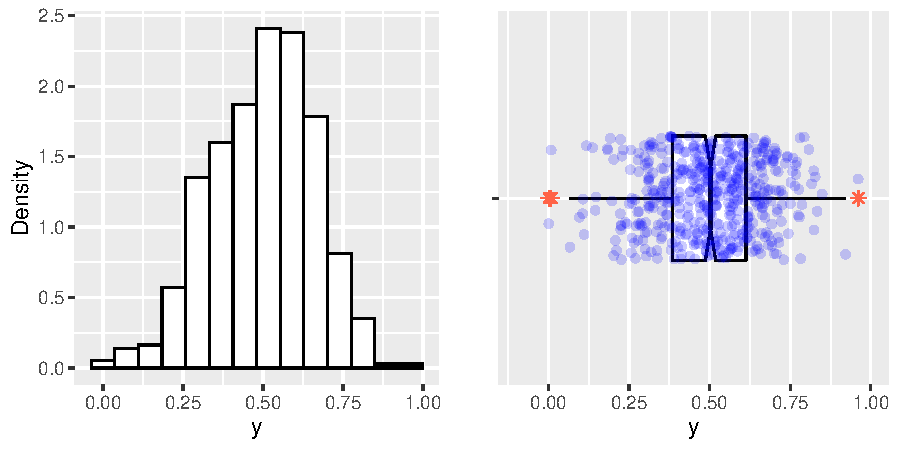
\includegraphics[width=0.80\textwidth]{figures/data_example_1.pdf}}
\caption{\label{data_example_1} Histogram (left panel) and boxplot (rigth panel) for $n=500$ simulated data from model \eqref{mod_ex_1}.}
\end{figure}

\begin{figure}[htp]
\centering
\makebox{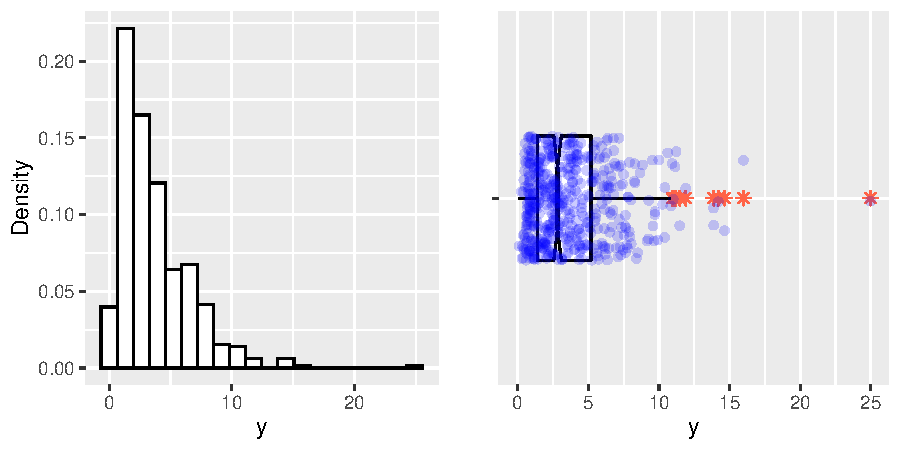
\includegraphics[width=0.80\textwidth]{figures/data_example_2.pdf}}
\caption{\label{data_example_2} Histogram (left panel) and boxplot (rigth panel) for $n=500$ simulated data from model \eqref{mod_ex_2}.}
\end{figure}

Using the simulated data shown in Figure \ref{data_example_1}, we fitted there models: Beta, Beta with bias correction and robust fitting model. Table \ref{res_example_1} contains the estimated parameters for $\mu$ and $\sigma$, the last line shows the true values for those parameters. From this table we note that the estimations for the robust fitting model are closer to the true values $\mu=5$ and $\sigma=5$. Additionally, the robust fitting model presents the lower AIC (Akaike Information Criterion) value.

\begin{table}[ht] 
\centering
\begin{tabular}{lccc} \hline
Model & $\mu$ & $\sigma$ & AIC \\ \hline
Beta & 3.90 & 4.00 & -376.35 \\ 
Beta with bias correction & 4.64 & 4.67 & -368.22 \\ 
Robust Beta & 4.89 & 4.91 & -462.07 \\ 
True & 5.00 & 5.00 & -- \\ \hline
\end{tabular}
\caption{Estimated values for $\mu$ and $\sigma$ under Beta, Beta with bias correction and robust fitting model. Last column presents the AIC (Akaike Information Criterion) and last line contains the true values for $\mu$ and $\sigma$ parameters.}
\label{res_example_1}
\end{table}

Using the simulated data shown in Figure \ref{data_example_2}, we fitted two models: ExGaussian and robust beta model. Table \ref{res_example_2} contains the estimated parameters for $\mu$, $\sigma$ and $\nu$, the last line shows the true values for those parameters. From this table we note that the estimations for the robust fitting model are closer to the true values $\mu=0.5$, $\sigma=0.1$ and $\nu=3$.

\begin{table}[ht]
\centering
\begin{tabular}{lcccc}
  \hline
Model & $\mu$ & $\sigma$ & $\nu$ & AIC \\ \hline
ExGaussian & 0.48 & 0.18 & 3.16 & 2208.98 \\ 
Robust ExGaussian & 0.48 & 0.15 & 3.12 & 2179.49 \\ 
True & 0.50 & 0.10 & 3.00 & -- \\ \hline
\end{tabular}
\caption{Estimated values for $\mu$, $\sigma$ and $\nu$ under ExGaussian and Robust ExGaussian. Last column presents the AIC (Akaike Information Criterion) and last line contains the true values for $\mu$, $\sigma$ and $\nu$ parameters.}
\label{res_example_2}
\end{table}

Figure \ref{3plots_both_examples} shows three plots to explore the results in a graphical way. The firts row contains the results for the Beta example and the second row the results for the ExGaussian example. Firts we analize the results for the Beta example shown in first row of the figure. In the left panel there are the estimated density $f(y)$ curves under Beta, Beta with bias correction and robust fitting model, it is clear that green curve explains better the observed pattern in the histogram and this curve is closer to the the gray line that represents the true density. In the middle panel we observe the estimated cumulative $F(y)$ curves under the fitted models with the empirical cumulative density function represented by small gray dots. With careful observation, we can notice that the red curve moves away from the empirical cumulative density function. In the right panel there are the estimated hazard function $h(y)$ under Beta, Beta with bias correction and robust fitting models. From this plot we note that green and gray curves overlap each other. From this figure we can conclude that the robust fitting explains better the pattern for the simulated and contaminated data. Similar patterns are observe for the ExGaussian example shown in the second row of the Figure \ref{3plots_both_examples}.

\begin{figure}[htp]
\centering
\makebox{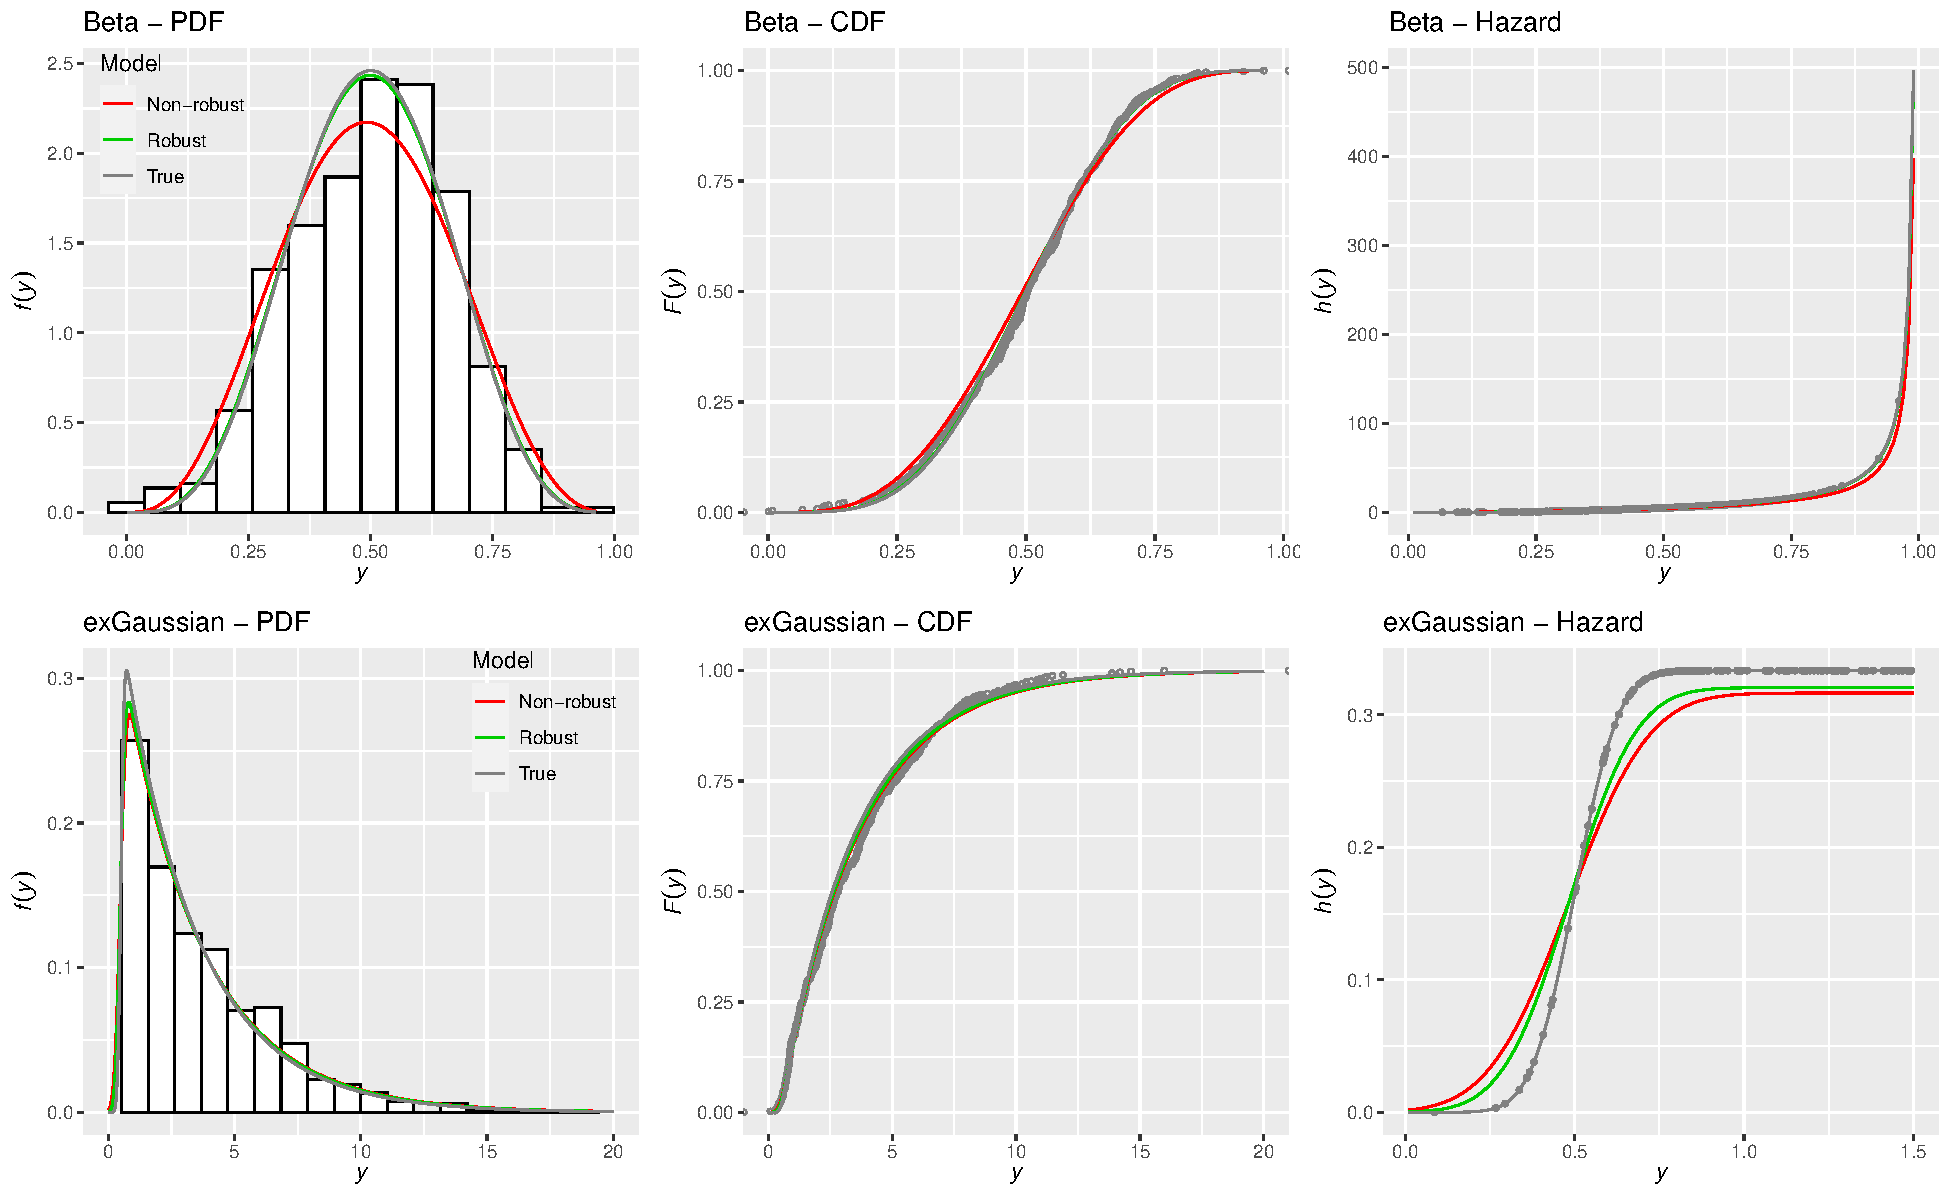
\includegraphics[width=1.00\textwidth]{figures/3plots_both_examples.pdf}}
\caption{\label{3plots_both_examples} Estimated $f(y)$, $F(y)$ and $h(y)$ for Beta and exGaussian examples.}
\end{figure}

Figure \ref{wp_both_examples} shows the worm plot proposed by \cite{buuren2001worm} which provides a guide to the adequacy of the fitted model. The worm plots for the robust fitting show a better pattern indicating that the robust fitting model is adequate for the data in both examples, Beta and ExGaussian.

\begin{figure}[htp]
\centering
\makebox{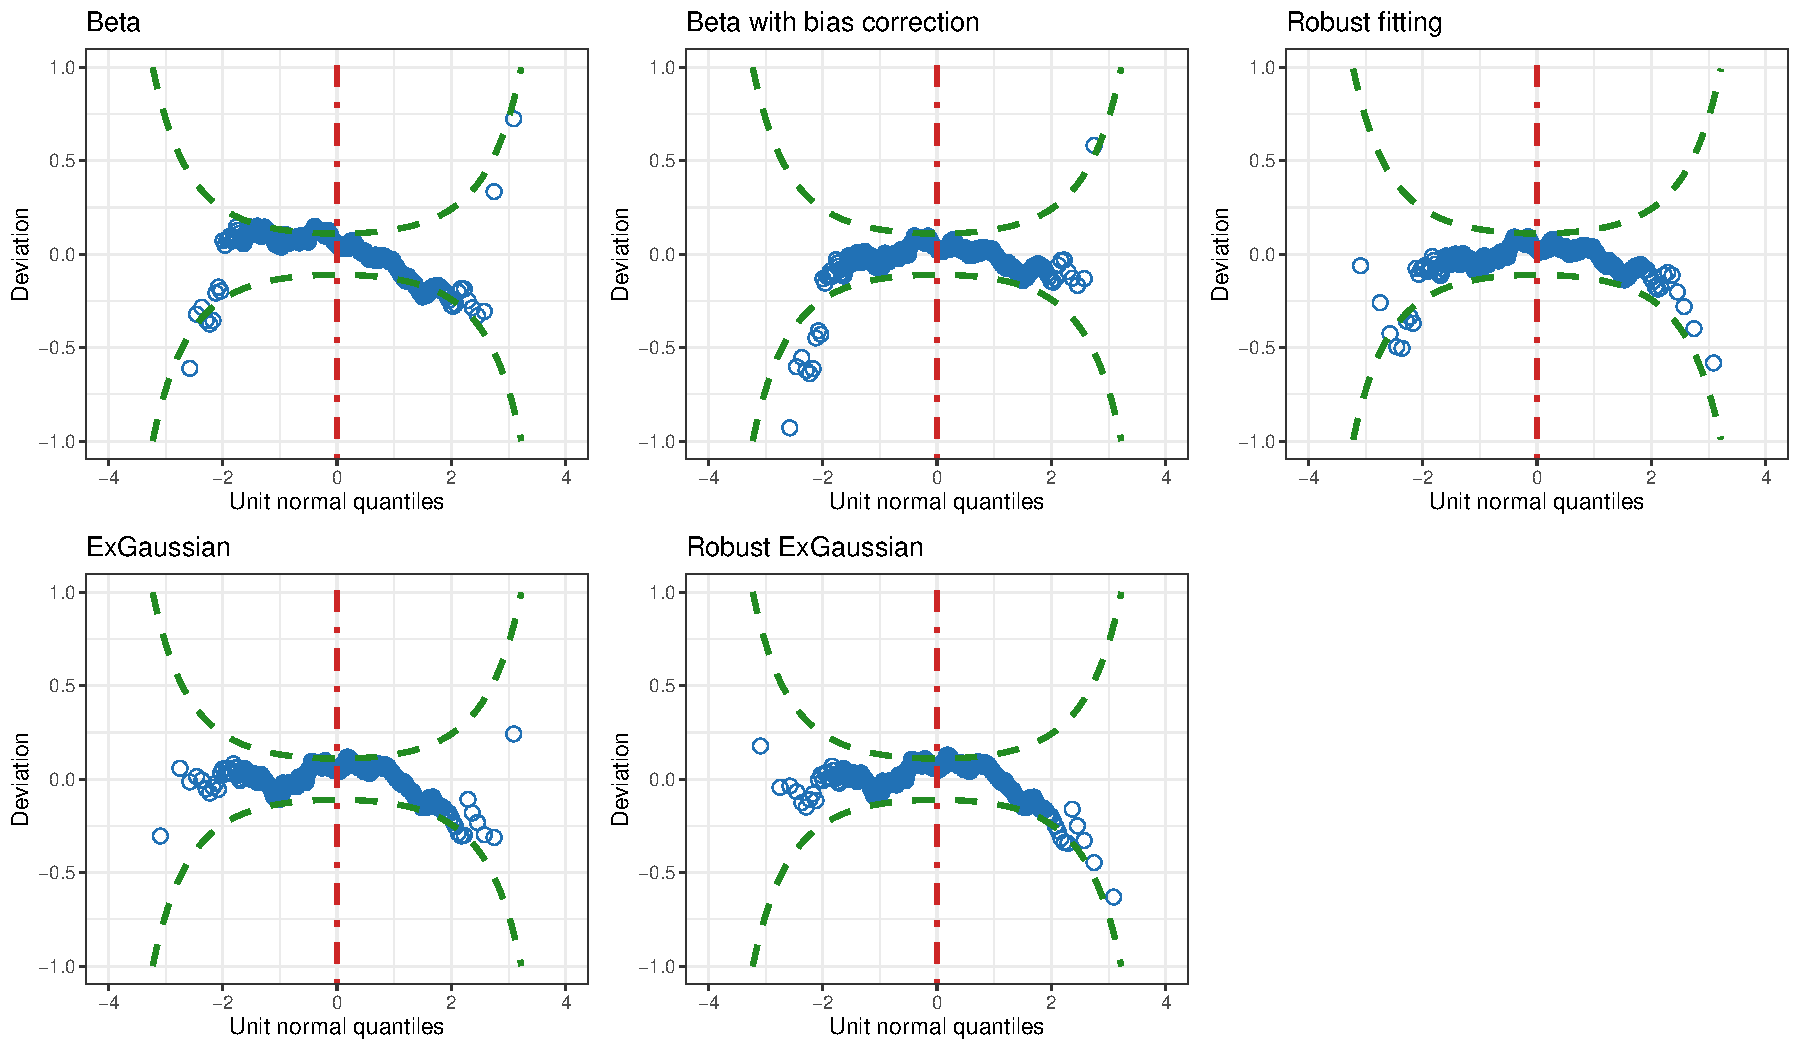
\includegraphics[width=1.00\textwidth]{figures/wp_both_examples.pdf}}
\caption{\label{wp_both_examples} Worm plots for Beta and exGaussian examples.}
\end{figure}

The R codes to replicate both examples presented in this section can be found in a github repository that can be found in this url \url{https://raw.githubusercontent.com/fhernanb/dist_gamlss_book/main/Robust%20estimation/Example%201%20%26%202.R}.
    
%-------------------------------------------------------------------
\bibliography{references}
%-------------------------------------------------------------------

\end{document} % This is the end of the document